\documentclass[]{beamer}
\mode<presentation>
% Time-stamp: <2014-11-10 17:56:39 (jonah)>

% beamer stuff
% Gives us the bottom line with all the goodies
\useoutertheme{infolines}
% Just the theme to use. Should be built into bemaer. Setting the
% height gets rid of a whole lot of whitespace
\usetheme[height=7mm]{Rochester}
\usefonttheme{serif}
% Usually beamer gives you navigation hyperlinks on the bottom
% right. I turned this off. It's annoying.
\setbeamertemplate{navigation symbols}{} 
% Makes my text boxes look pretty
\setbeamertemplate{blocks}[rounded][shadow=true] 
% Makes my bullet points 3d balls
\setbeamertemplate{items}[ball]

% Packages 
\usepackage{rotating}
\usepackage{multimedia}
\usepackage{tabularx}
\usepackage{booktabs}
\usepackage{subfigure}
\usepackage{graphicx}
\usepackage{mathrsfs}
\usepackage{amsmath}
\usepackage{amssymb}
\usepackage{latexsym}
\usepackage{amsfonts}
\usepackage[mathscr]{eucal}
\usepackage{mathrsfs}
\usepackage{verbatim}
\usepackage{braket}
\usepackage{listings}
\usepackage{amsthm}
\usepackage{color}
\usepackage{fancybox}
\usepackage{animate}
\usepackage{multicol}
\usepackage{mdframed}
\usepackage{braket}
\usepackage{multicol}

% for counter control
\usepackage{lipsum}

% Macros

%Blackboard Bold
\newcommand{\R}{\mathbb{R}}
\newcommand{\Z}{\mathbb{Z}}
\newcommand{\N}{\mathbb{N}}
\newcommand{\Q}{\mathbb{Q}}
\newcommand{\A}{\mathbb{A}}
\newcommand{\E}{\mathbb{E}}
% other
\newcommand{\eval}{\biggr\rvert} %evaluated at
\newcommand{\myvec}[1]{\mathbf{#1}} % vectors for me
% total derivatives 
\newcommand{\diff}[2]{\frac{d #1}{d #2}} 
\newcommand{\dd}[1]{\frac{d}{d #1}}
% partial derivatives
\newcommand{\pd}[2]{\frac{\partial #1}{\partial #2}} 
\newcommand{\pdd}[1]{\frac{\partial}{\partial #1}} 

% Lets you not count frames for backup slides
\newcommand{\backupbegin}{
   \newcounter{finalframe}
   \setcounter{finalframe}{\value{framenumber}}
}
\newcommand{\backupend}{
   \setcounter{framenumber}{\value{finalframe}}
}

\title[spectral]{An Introduction to Spectral Methods in Python}
\author[J. Miller]{Jonah M. Miller}
\institute[PI]{Perimeter Institute}

\date[November 2014]{Tuesday, November 4, 2014}

\begin{document}

\begin{frame}[plain]
\titlepage
\end{frame}

% \begin{frame}
%   \frametitle{Spectral Methods Vs. Advantages and Disadvantages.}
%   \begin{columns}
%     \column{6cm}
%     \begin{center}{\Large\underline{Advantages}}\end{center}
%     \begin{itemize}
%     \item Error falls off exponentially with increased reasolution
%     \item Compare this to finite differences, where the error falls off
%       as $h^n$
%       \item Mathematically very elegant
%     \end{itemize}
%     \column{6cm}
%     \begin{center}{\Large\underline{Disadvantages}}\end{center}
%     \begin{itemize}
%     \item Computational cost grows quadratically with increased resolution
%     \item Compare to finite differences, where computational cost
%       grows linearly with resolution.
%     \item Good only for smooth solutions. Cannot handle shocks.
%     \item Geometrically inflexible. 
%     \end{itemize}
%   \end{columns}
% %     \begin{block}{Note:}
% %       There exist hybrid methods (e.g., \textit{discontinuous Galerkin}
% %         methods) that combine the strengths of spectral methods with
% %       the strengths of shock-capturing methods.
% %     \end{block}
% \end{frame}

\begin{frame}
  \frametitle{The Method of Lines}
  \begin{itemize}
    \item Suppose we want to solve the linear advection equation:
      $$\pd{u}{t} = c \pd{u}{x}$$
    \item Discretize \textit{space only}
      $$\pdd{t}{u_i(t)} = c \frac{u_i(t) - u_{i-1}(t)}{\Delta x}$$
    \item This is a \textit{coupled system} of ODEs:
      $$\pdd{t}\myvec{u} = D \myvec{u},\text{ for some matrix }D$$
    \item Solve using ODE methods discussed earlier such as RK2
  \end{itemize}
\end{frame}

\begin{frame}
  \frametitle{What do we Discretize?}
  \pause
  \setlength{\unitlength}{1 cm}
  \begin{picture}(11,8)
    \put(1,7){\huge \underline{Equation}}
    \put(1,5.){\Large $\pd{u}{t} + c \pd{u}{x}=0$}
    \color{red}
    \thicklines
    \put(2.3,4.75){\vector(0,-1){2}}
    \color{black}
    \put(0.25,2.){\Large $\frac{u_i^{n+1} - u_{i}^n}{\Delta t} + c \frac{u_{i}^n - u_{i-1}^n}{\Delta x} = 0$}
    \put(7.,4.5){\includegraphics[width=4cm]{smooth-solution.png}}
    \put(8,7){\huge\underline{Function}}
    \put(7.,1){\includegraphics[width=4cm]{linear-spline.png}}
    \color{red}
    \put(9.3,4.75){\vector(0,-1){2}}
  \end{picture}
\end{frame}

\begin{frame}
  \frametitle{Discretizing the Solution: The Function-Space Picture}
  \begin{itemize}
    \item Represent solution as infinite-dimensional  vector in Sobolev space
      $$u(x) = \sum_{i=0}^\infty u_i \phi_i(x)$$
    \item To approximate, restrict to finite-dimensional subspace:
      $$u(x) \approx \tilde{u}(x) = \sum_{i=0}^N u_i \phi_i(x)\text{ where }N\in\N$$
  \end{itemize}
\end{frame}

\begin{frame}
  \frametitle{A Legendre Basis}
  \begin{center}
    \vspace{-0.5cm}
    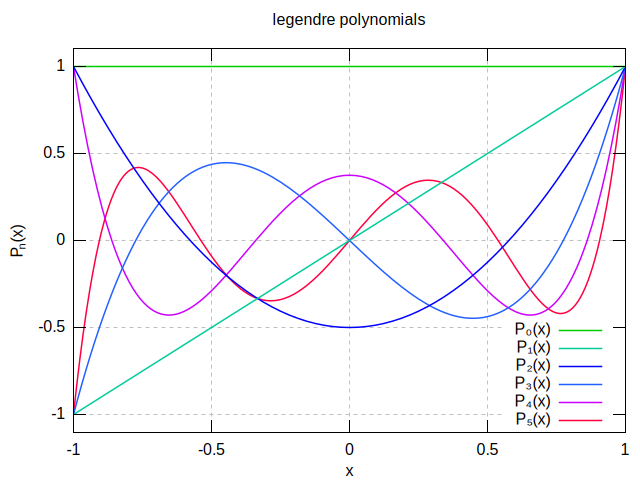
\includegraphics[width=11cm]{Legendrepolynomials6.png}
  \end{center}
  \vspace{-0.5cm}
  Source: Wikipedia
\end{frame}

\begin{frame}
  \frametitle{A Chebyshev Basis}
  \begin{center}
    \vspace{-0.3cm}
    \hspace{-0.6cm}
    \includegraphics[width=12.5cm,height=8.75cm]{chebyshev_polynomials_jmm.png}
    %\includegraphics[width=11cm]{Chebyshev_Polynomials_of_the_1st_Kind.png}
  \end{center}
\end{frame}


\begin{frame}
  \frametitle{Finite Differences in the Function Space Picture}
  \setlength{\unitlength}{1 cm}
  \begin{picture}(11,8)
    \put(6,7){\large $\phi_i$ are simple piecewise functions}
    \thicklines
    \put(0,5){\line(1,0){2}}
    \put(2,5){\line(1,1){2}}
    \put(4,7){\line(1,-1){2}}
    \put(6,5){\line(1,0){6}}
    \put(0,1){\line(1,0){4}}
    \put(4,1){\line(1,1){2}}
    \put(6,3){\line(1,-1){2}}
    \put(8,1){\line(1,0){4}}
    \color{red}
    \multiput(0,5)(2,0){7}{\circle*{0.5}}
    \multiput(0,1)(2,0){7}{\circle*{0.5}}
  \end{picture}
%   \begin{itemize}
%     \item Break total sum into two:
%       $$u(t,x) = \sum_{i=0}^N\sum_{j=0}^1 u_{ij}(t) \phi_{ij}(x)$$
%     \item Where 
%       $$\begin{cases}\phi_{i0}=m_i x\chi_i(x)\\\phi_{i1}=b_i\chi_i(x)\end{cases}\text{ where }\chi_i(x)=\begin{cases}1&\text{ if }x\in[x_i,x_i+1]\\0&\text{ otherwise}\end{cases}$$
%       \item Such that $u(t,x)$ between points $x_i$ and $x_{i+1}$ is of the form
%         $$u = m_ix + b_i$$
%   \end{itemize}
%   \pause
%   \begin{Large}
%     \begin{center}
%       Notice how redundant this is!
%     \end{center}
%   \end{Large}
\end{frame}

% \begin{frame}
%   \frametitle{Choice Basis Functions: Orthogonal Functions}
%   \begin{Large}$$\braket{\phi_i,\phi_j} = \int_{a}^b \phi_i(x)\phi_j(x) w(x) dx = \delta_{ij}$$\end{Large}
%   \begin{itemize} 
%   \item A Fourier basis works well for periodic boundary conditions:
%     $$[a,b]=[-\pi,\pi]\text{ and }w(x) = 1$$
%   \item Chebyshev Polynomials minimize the Gibbs phenomenon and are
%     compatible with all boundary conditions:
%     $$[a,b]=[-1,1]\text{ and }w(x) = (1-x^2)^{\pm 1/2}$$
%   \item Legendre polynomials minimize numerical error when converting
%     a spectral representation to a polynomial interpolation (more later).
%     $$[a,b]=[-1,1]\text{ and }w(x) = 1$$
%   \end{itemize}
% \end{frame}

% \begin{frame}
%   \frametitle{Precision Quadrature and the Inner Product}
%   \begin{block}{Theorem}
%     For all $f\in\mathbb{P}_{2N + \delta}$, there exist $N+1$ positive
%     real numbers $x_n$ in the domain $\Omega$ such that:
%     $$\int_\Omega f(x) w(x) dx = \sum_{n=0}^Nf(x_n) w_n,$$
%     where $w_n$ are discrete weights that may be different from the
%     original weight function and where $\delta$ is an integer that
%     depends on the precise choice of $w_n$. (Usually, $\delta\in\{-1,0,1\}$.)
%   \end{block}
%   \pause
%   \begin{block}{Application}
%     This lets us precisely calculate the inner product between our
%     grid function $u$ and basis elements (or test functions)
%     $\phi_i$!
%   \end{block}
% \end{frame}

\begin{frame}
  \frametitle{Approximating the Equation}
  \begin{itemize}
%   \item A residual $\mathcal{R}$ is a function of the numerical
%     solution that measures how well it solves the original
%     equation. Usually we demand that the residual vanishes.
    \item E.g., for 
      $$\pd{u}{t} + c \pd{u}{x}=0,$$
  \end{itemize}  
  \begin{block}{In Finite Differences, demand:}
    $$\frac{u_i^{n+1} - u_{i}^n}{\Delta t} + c \frac{u_{i}^n - u_{i-1}^n}{\Delta x} = 0\ \forall\ i,n\in\Z$$
  \end{block}
  \begin{block}{In Galerkin Methods, Demand:}
    $$\int_a^b \left(\pd{\tilde{u}}{t} + c \pd{\tilde{u}}{x}\right)\phi_i \; w \; dx = 0\ \forall\ i\in\N$$
  \end{block}
\end{frame}


\begin{frame}
  \frametitle{Measuring Goodness}
  \begin{columns}
    \column{6cm}
    \begin{center}{\Large\underline{Error}}\end{center}
    \begin{center}
      $$\epsilon(t,x) = u(t,x) - \tilde{u}(t,x),$$
      $$\text{ where }L[u] = 0$$
      $$\text{generically, }\epsilon(x) > 0$$
    \end{center}
    \column{6cm}
    \begin{center}{\Large\underline{Residual}}\end{center}
    \begin{center}
      $$R(t,x) = \tilde{L}[\tilde{u}]$$
      $$\text{often demand that}$$
      $$\mathcal{R}(t,x) = 0\text{ identically }$$
    \end{center}
  \end{columns}
\end{frame}

\begin{frame}
  \frametitle{Measuring Goodness}
  \begin{columns}
    \column{6cm}
    \begin{center}{\Large\underline{Error}}\end{center}
    \begin{center}
      $$\epsilon_i^n = u(t,x)\eval^{t=t^n}_{x=x^i} - u_i^{n+1},$$
      $$\text{ or }$$
      $$\epsilon_i^n = \left[\int_a^b\left(u(t,x) - \tilde{u}(t,x)\right)\phi_i dx\right]_{t=t^n}$$
      $$\text{generically, }\epsilon_i^n > 0$$
    \end{center}
    \column{6cm}
    \begin{center}{\Large\underline{Residual}}\end{center}
    \begin{center}
      $$\mathcal{R}_i^n = \frac{u_i^{n+1} - u_{i}^n}{\Delta t} + c \frac{u_{i}^n - u_{i-1}^n}{\Delta x}$$
        $$\text{or}$$
        $$\mathcal{R}_i^n = \left[\int_a^b\left(\pd{\tilde{u}}{t}+c\pd{\tilde{u}}{x}\right)\phi_idx\right]_{t=t^n}$$
      $$\text{often demand that}$$
      $$\mathcal{R}_i^n = 0\text{ identically }\forall\ i,n\in\N $$
    \end{center}
  \end{columns}
\end{frame}


% \begin{frame}
%   \frametitle{Recovering A Numerical Scheme (part 1)}
%   \begin{itemize}
%     \item Suppose we want to solve the following equation on the domain $[-1,1]$:
%       $$\pdd{t}u+c\pdd{x} u(x) = 0$$
%       \pause
%     \item Then for a given $N\in\N$ we assume our solution is of the form
%       $$u(t,x)=\sum_{i=0}^N u_i \phi_i(x),\text{ where }u_i \in\R$$
%       \pause
%     \item We form a residual and demand that it vanish for all basis functions $\phi_i$:
%       $$\mathcal{R} = \int_{-1}^1 \left(\pd{u}{t} + c\pdd{u}{x}\right)\phi_i(x)dx=0\ \forall\ i$$
%   \end{itemize}
% \end{frame}
% 
% \begin{frame}
%   \frametitle{Recovering A Numerical Scheme (part 2)}
%   \begin{itemize}
%   \item If we plug our ansatz for $u$ into the residual and integrate by parts, we find:
%     $$\sum_{j}\mathcal{M}_{ij}\pd{u_j}{t} - c \sum_{j}\mathcal{S}_{ij}u_j + B_j =0,$$
%     where
%     $$\mathcal{M}_{ij} = \int_{-1}^1\phi_i\phi_j dx$$
%     is the \textit{mass matrix},
%     $$\mathcal{S}_{ij} = \int_{-1}^1\phi_i\pd{\phi_j}{x}dx$$
%     is the \textit{stiffness matrix}, and $B_j$ is some vector of
%     boundary terms.
%     \pause
%   \item Invert $\mathcal{M}$ and solve for $u_i$ coefficients to get a
%     system of coupled ODEs that can be integrated forward in time
%     using ODE methods.
%   \end{itemize}
% \end{frame}
% 
% \begin{frame}
%   \frametitle{A Simple Numerical Example}
%   \begin{center}
%     \begin{huge}
%       Open up the \textit{linear-advection} IPython notebook for a
%       simple example where we solve the linear advection equation with a
%       spectral method.
%     \end{huge}
%   \end{center}
% \end{frame}
% 
% \begin{frame}[plain]
%   \begin{center}
%     {\huge Pseudospectral Methods}
%   \end{center}
% \end{frame}
% 
% \begin{frame}
%   \frametitle{A Generalization of Spectral Methods}
%   \pause
%   \begin{itemize}
%     \item A ``wave'' description means spectral methods are generically highly non-local.
%     \item This makes solving nonlinear equations (where local values
%       of the solution matter) very complicated.
%       \pause
%     \item To solve this problem, we represent the function locally (in
%       a similar way to finite differences) but transform to a spectral
%       representation to take derivatives.
%   \end{itemize}
% \end{frame}
% 
% \begin{frame}
%   \frametitle{Polynomial Interpolation}
%   \begin{itemize}
%   \item Suppose a set of $N+1$ points $\{x_i\}_{i=0}^N$ such that
%     $x_{i+1}>x_i$ and a numerical solution $u(x_i)$ defined on those
%     points
%     \pause
%   \item Then an \textit{interpolating polynomial} is the unique polynomial of order $N$,
%     $$p(x) = \sum_{i=0}^N a_i x^i$$
%     such that
%     $$p(x_i) = u(x_i).$$
%   \end{itemize}
% \end{frame}
% 
% \begin{frame}
%   \frametitle{Nodal and Modal Representations}
%   \begin{columns}
%     \column{6cm}
%     \begin{center}{\Large\underline{Nodal}}\end{center}
%     \begin{itemize}
%     \item Represent $u(t,x)$ as a value on a discrete grid: $u_i=u(x_i)$
%     \item Discrete representation is a vector $\myvec{u}=[u(x_0),u(x_1),...,u(x_N)]$
%     \item Use polynomial interpolation to extract global solution on $[x_0,x_N]$
%     \item $\mathcal{R}_i=f(u(x_i))$ can be made to be local to $x_i$
%     \end{itemize}
%     \column{6cm}
%     \begin{center}{\Large\underline{Modal}}\end{center}
%     \begin{itemize}
%     \item Represent $u(t,x)$ as sum over polynomial basis functions: $u(t,x)=\sum c_i(t) \phi_i(x)$
%     \item Discrete representation is a vector $\myvec{c}=[c_0,c_1,...,c_N]$
%     \item $\mathcal{R}_i=f(u,\phi_i)$ is highly nonlocal
%     \end{itemize}
%   \end{columns}
% \end{frame}
% 
% \begin{frame}
%   \frametitle{Combining Nodes and Modes}
%   \begin{itemize}
%   \item Represent the \textit{same} solution \textit{both} nodally and
%     modally.
%     \pause
%   \item The interpolating polynomial $p_t(x)$ is \textit{unique}
%     \pause
%   \item Therefore,
%     $$p_t(x) = u(t,x) = \sum_{i}c_i \phi_i(x)$$
%     \pause
%   \item Therefore \textit{there exists a transformation between the
%       nodal and modal representations.}
%   \end{itemize}
% \end{frame}
% 
% \begin{frame}
%   \frametitle{The Pseudospectral Strategy}
%   \begin{itemize}
%     \item Represent our function and impose boundary conditions nodally 
%     \item Transform to the modal representation to take derivatives
%     \item Transform back.
%   \end{itemize}
% \end{frame}
% 
% \begin{frame}
%   \frametitle{Colocation Points}
%   
% \end{frame}

% \begin{frame}
%   \frametitle{Polynomial Interpolants and Orthogonal Polynomials}
%   \begin{itemize}
%   \item Suppose that we have a set points $\{x_i\}_{i=0}^N$ where we
%     wish our solution $u(t,x_i)$ to be \textit{exact}. 
%     \pause
%   \item We can represent our solution as a vector
%     $\myvec{u}_t=[u(t,x_0),u(t,x_1),...,u(t,x_N)]$ where $u_i=u(t,x_i)$.
%     \pause
%   \item To find $u$ between the $x_i$ points,use an $N^{th}$ order
%     polynomial interpolant $p_t(x)$, where subscript reminds us that
%     we have a different polynomial at each time $t$.  
%     \pause
%   \item Suppose further that we would \textit{also} like to represent
%     $u$ as a finite sum of orthogonal polynomials: $u(t,x) = \sum_{i}c_i(t) \phi_i.$
%     \pause
%   \item Then because the interpolating polynomial is \textit{unique}, 
%     $$p_t(x)=\sum_{i}c_i(t)\phi_i.$$
%     \pause
%   \item Therefore, there exists a \textit{transformation} between the 
%     \end{itemize}
% \end{frame}

% \begin{frame}
%   \frametitle{Colocation Points}
%   \pause
%   \begin{itemize}
%   \item Suppose we want to represent our function as an interpolating polynomial because for a 
%   \item Suppose we have a basis of orthogonal polynomials
%     $\{\phi_i\}_{i=0}^N$, and a representation of our solution $u$,
%       $$u(t,x) = \sum_{i=0}^N u_i(t) \phi_i(x).$$
%       \pause
% 
%     \item Then it is \textit{always} possible to choose a set of
%       \textit{colocation points} $\{x_i\}_{i=0}^N$ such that $u(t
%   \end{itemize}
% 
% \end{frame}

\begin{frame}
  \frametitle{Example: The Galerkin Scheme}
  Suppose we want to solve
  $$\pd{u}{t} +\pdd{x} F[u] = 0$$
  where $F$ is an arbitrary (\textit{nonlinear}) functional of $u$
  using the ansatz:
  $$u(t,x) \approx \tilde{u} = \sum_{i=1}^N u_i(t) \phi_i(x)\ N\in\N$$
  and
  $$F[u] \approx \tilde{F} = \sum_{i=1}^N F_i[u] \phi_i(x)$$
\end{frame}

\begin{frame}
  \frametitle{Exercise}
  \begin{itemize}
  \item Solve the equation
    $$\pd{u}{t} + c \pd{u}{x} = 0\text{ with }u(0,x)=\sin\left(e^{-(x-\pi)^2}\right)\text{ for }x\in[-\pi,\pi]$$
    with periodic boundary conditions.
  \item Use a Fourier ansatz:
    $$u(t,x) = a_0 + \sum_{k=1}^N \left[a_k(t) \cos(kx) + b_k(t) \sin(kx)\right]\text{ for some }N\in\N$$
    \item Assume the following inner product:
      $$\braket{a,b} = \frac{1}{\pi}\int_{-\pi}^{\pi}a(x) b(x) dx$$
  \end{itemize}
\end{frame}

\begin{frame}
  \frametitle{Resources}
  {\Large\underline{In no particular order:}}
  \vspace{1cm}
  \begin{itemize}
    \item \textit{Numerical Recipes}, by Press, Teukolsky, Vetterling, and Flannery
    \item \textit{Scientific Computing: An Introductory Survey}, by Heath
    \item \textit{Introduction to Spectral Methods}, by Grandclement (\href{http://arxiv.org/abs/gr-qc/0609020}{arXiv:gr-qc/0609020}).
    \item \textit{Spectral Methods in MATLAB}, by Trefethen
  \end{itemize}
\end{frame}

\end{document}